\begin{problem}
Let $X$ be a Hausdorff space and let $A$ be a compact subset of
$X$. Prove from the definitions that $A$ is closed.
\end{problem}
\begin{proof}
This is Theorem 26.3 from Munkers \S26, p.\,165; we shall paraphrase it.
\\\\
We show that $X-A$ is open. To that end we will show that, given a point
$x_0\in X-A$, there is neighborhood $U$ of $x_0$ disjoint from $A$. For
each point $a\in A$, by the Hausdorff property of $X$, choose disjoint
neighborhoods $U_a$ and $V_a$ of $x_0$ and $a$, respectively. Then the
collection $\left\{\,V_a\;\middle|\;a\in A\,\right\}$ forms an open cover
of $A$ so, by Lemma 26.1, only finitely many of the $V_a$'s cover $A$, say
$V_{a_1},...,V_{a_n}$. Define $U\coloneqq U_{a_1}\cap\cdots\cap
U_{a_n}$. We claim that $U$ is a neighborhood of $x_0$ disjoint from
$A$. First, it is clear that $U$ is a neighborhood of $x_0$ since each
$U_a$ contains $x_0$ and $U$ is an intersection of finitely many of
these. Second, note that if $z\in U\cap A$ then $z\in U_{a_i}$ for all $i$
and $z\in V_{a_j}$ for some $j\in\{1,...,n\}$, but $U_{a_j}\cap
V_{a_j}=\emptyset$. Therefore, $U\cap A=\emptyset$. By Lemma C, it follows
that $X-A$ is open.
\end{proof}
\begin{problem}
Let $X$ be a Hausdorff space and let $A$ and $B$ be disjoint
compact subsets of $X$. Prove that there are open sets $U$ and
$V$ such that $U$ and $V$ are disjoint, $A\subset U$ and
$B\subset V$.
\end{problem}
\begin{proof}
This is Ex.\,5 from Munkres \S26, p.\,171.
\\\\
Suppose $A$ and $B$ are disjoint compact subspaces of $X$. Since $X$ is
Hausdorff, by Theorem 26.4, for every $x\in B$ there exists disjoint open
sets $U_x$ and $V_x$ where $U_x\supset A$ and $V_x$ is a neighborhood of
$x$. Then the collection $\left\{\,V_x\;\middle|\;x\in B\right\}$ is an
open cover of $B$ so by Lemma 26.1, only finitely many of the $V_x$'s cover
$B$, say $V_{x_1},...,V_{x_n}$. Define $U\coloneqq U_{x_1}\cap\cdots\cap
U_{x_n}$ and $V\coloneqq V_{x_1}\cup\cdots\cup V_{x_n}$. We claim that $U$
and $V$ are disjoint neighborhood containing $A$ and $B$, respectively. It
is clear that $U$ and $V$ are open since $U$ is a finite intersection of
open sets and $V$ is a union of open sets and that they contain $A$ and
$B$, respectively, since each of the $U_x$'s contain $A$ and
$V_{x_1},...,V_{x_n}$ is an open cover of $B$. Lastly, $U$ and $V$ are
disjoint since intersection distributes over union, i.e., we have
\[
U\cap V=
\left(\bigcap_{i=1}^nU_{x_i}\right)\cap\left(\bigcup_{j=1}^n
  V_{x_j}\right)=
\bigcup\left(\bigcap_{i=1}^nU_{x_i}\cap V_{x_j}\right)=\emptyset
\]
since $U_{x_i}\cap V_{x_i}=\emptyset$ so
$\left(\bigcap_{i=1}^nU_{x_j}\right)\cap V_{x_i}=\emptyset$.
\end{proof}
\begin{problem}
Prove the Tube Lemma: Let $X$ and $Y$ be topological spaces with
$Y$ compact, let $x_0\in X$, and let $N$ be an open set of
$X\times Y$ containing $x_0\times Y$, then there is an open set
$W$ of $X$ containing $x_0$ with $W\times Y\subset
N$.
\end{problem}
\begin{proof}
This is Lemma 26.8 from Munkres \S26, p.\,168, but is proved in \emph{Step
  1} in the process of showing Theorem 26.7; we paraphrase the proof here.
\\\\
Let $x_0\in X$, and let $N$ be an open set of $X\times Y$ containing
$x_0\times Y$. Cover $x_0\times Y$ by basic open sets $U\times V$ lying in
$N$. Note that $x_0\times Y$ is compact, since it is an imbedding of $Y$
given by the map $y\mapsto (x_0,y)$ from $Y$ into $X\times Y$ therefore, by
Lemma 26.1, only finitely many of the $U\times V$'s, say $U_1\times
V_1,...,U_n\times V_n$, cover $x_0\times Y$. Define $W\coloneqq
U_1\cap\cdots\cap U_n$. We claim that $W$ is a neighborhood of $x_0$ such
that $W\times Y\subset N$. First, it is clear that $W$ is a neighborhood of
$x_0$ since it is the finite intersection of open sets and each $U_i\times
V_i$ intersects $x_0\times Y$ hence contains a point of the form $(x_0,y)$
so $U_i=\pi_1(U_i\times V_i)$ contains $x_0$. Lastly, $W\times Y\subset N$
since $W\times Y\subset\bigcup_{i=1}^n U_i\times V_i$. To see this let
$(x,y)\in W\times Y$ and consider the point $(x_0,y)\in x_0\times Y$. Since
$(x_0,y)$ is in $U_i\times V_i$ for some $i$, we have $y\in V_i$. But $x\in
U_j$ for every $j$ since $x\in W$. Thus $(x,y)\in U_i\times V_i$ as
desired. It follows that, $W$ is a neighborhood of $x_0$ with $W\times
Y\subset N$ as desired.
\end{proof}
\begin{problem}
Show that if $Y$ is compact, then the projection map $X\times
X\to X$ is a closed map.
\end{problem}
\begin{proof}
We shall proceed by the tube lemma, i.e, Theorem 26.8. Let $C$ be a closed
subset of $X\times Y$ then $N=(X\times Y)-C$ is open. Choose $x_0\in
X-\pi_1(C)$. Then $x_0\times Y$ is contained in $N$ so by the tube lemma,
there exists a neighborhood $W$ of $x_0$ such that $W\times
Y\subset N$. In particular, $W\subset X-\pi_1(C)$ otherwise if
$x\in W\cap\pi_1(C)$ then $x\times Y\subset N$ and $(x,y)\in C$
for some $y\in Y$, but $N\cap C=\emptyset$. It follows by Lemma C
that $X-\pi_1(C)$ is open so $\pi_1(C)$ is closed. Since $C$ was
chosen arbitrarily we see that $\pi_1$ is a closed map.
\end{proof}
\begin{problem}
Let $X$ be a compact space and suppose we are given a nested
sequence of subsets $C_1\supset C_2\supset\cdots$ with all $C_i$
closed. Let $U$ be an open set containing $\bigcap C_i$. Prove
that there is an $i_0$ with $C_{i_0}\subset U$.
\end{problem}
\begin{proof}
Consider the family of open sets $U_i\coloneqq X-C_i$. Since $U$
is open $X-U$ is closed so by Theorem 26.2 is compact. We claim
that $U_i$ forms an open cover of $X-U$. To see note that by De
Morgan's laws
\[
\bigcup_{i\in\NN} U_i=\bigcup_{i\in\NN} X-C_i=X-\bigcap_{i\in\NN}
C_i\supset X-U
\]
since $\bigcap_{i\in\NN} C_i\subset U$. Therefore by Lemma 26.1
only finitely many of the $U_i$'s cover $X-U$, say
$U_{i_1},...,U_{i_n}$. Thus, we have that $X-U\subset \bigcup_{i=1}^n
U_i$ so $U\supset\bigcap_{j=1}^n C_{i_j}=C_{i_n}$ as desired.
\end{proof}
\begin{problem}
Let $X$ be a compact space, and suppose there is a finite family
of continuous functions $f_i\colon X\to\RR$, $i=1,...,n$ with the
following property: given $x\neq y$ in $X$ there is an $i$ such
that $f_i(x)\neq f_i(y)$. Prove that $X$ is homeomorphic to a
subspace of $\RR^n$.
\end{problem}
\begin{proof}
Consider the map $f\colon X\to\RR^n$ defined by
$f\coloneqq(f_1,...,f_n)$. This map is continuous by Theorem 18.4
since each component $f_i$ is continuous. We claim that $X\approx
f(X)$. To prove this it suffices to show that $f$ is injective so
that its restriction to $f(X)$ will be surjective and lastly
invoke Theorem 26.6. Suppose $f(x)=f(y)$ but $x\neq y$. Then
$f_i(x)\neq f_i(y)$ for some $i$, but this implies that $f(x)\neq
f(y)$. This is a contradiction therefore, $x=y$. It follows that
$f$ is a bijection from a compact space $X$ into
$f(X)\subset\RR^n$ so by Theorem 26.6, we have $X\approx f(X)$.
\end{proof}
\begin{problem}
Let $X$ be a compact metric space and let $\mathcal{U}$ be a
covering of $X$ by open sets. Prove that there is an
$\varepsilon>0$ such that, for each set $S\subset X$ with
diameter $<\varepsilon$, there is a $U\in\mathcal{U}$ with
$S\subset U$. (This fact is known as the ``Lebesgue number lemma.'')
\end{problem}
\begin{proof}
This is Lemma 27.5 from Munkres \S27, p.\,175; we will paraphrase the
proof.
\\\\
Let $\mathcal{U}$ be an open cover of $X$. If $X\in\mathcal{U}$, then any
positive number is a Lebesgue number for $\mathcal{U}$. Suppose
$X\notin\mathcal{U}$. Choose a finite subcollection $U_1,...,U_n$ of
$\mathcal{U}$ that covers $X$. For each $i$, set $C_i\coloneqq X-U_i$ and
define the map $f\colon X\to\RR$ via
$f(x)\coloneqq\frac{1}{n}\sum_{i=1}^nd(x,C_i)$. We show that $f(x)>0$ for all
$x$. Given $x\in X$, choose $i$ so that $x\in U_i$. Then choose
$\varepsilon$ so that the $\varepsilon$-neighborhood of $x$ lies in
$U_i$. Then $d(x,C_i)\geq\varepsilon$, so that $f(x)\geq\varepsilon/n$.

Since $f$ is continuous, it has a minimum value $\delta$; we show that
$\delta$ is our required Lebesgue number. Let $B$ be a subset of $X$ of
diameter less that $\delta$. Choose a point $x_0$ of $B$; then $B$ lies in
a $\delta$-neighborhood of $x_0$. Now $\delta\leq f(x_0)\leq d(x_0,C_m)$,
where $d(x_0,C_m)$ is the largest of the numbers $d(x_0,C_i)$. Then the
$\delta$-neighborhood of $x_0$ is contained in the element $U_m=X-C_m$ of
the covering $\mathcal{U}$.
\end{proof}
\begin{problem}
Let $S^1$ denote the circle $\left\{\,x^2+y^2=1\,\right\}$ in
$\RR^2$. Define an equivalence relation on $S^1$ by
\[\text{$(x,y)\sim (x',y')$ $\iff$ $(x,y)=(x',y')$ or $(x,y)=(-x',-y')$}\]
(you do not have to prove that this is an equivalence
relation). Prove that the quotient space $S^1/{\sim}$ is
homeomorphic to $S^1$.

One way to do this is by using complex numbers.
\end{problem}
\begin{proof}
Since Dr.\,McClure said that we can assume anything from complex analysis
(and we don't need much) to begin with we shall assume that
$S^1\subset\CC$. Now, the situation is as follows we want to find a map
$f\colon S^1\to S^1$ which preserves $\sim$ that makes the following
diagram commute
\begin{center}
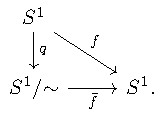
\includegraphics{figures/mid-2-rp-1-s-1}
\end{center}
Define $f(z)\coloneqq z^2$. We claim that $f$ is continuous and preserves
$\sim$. First, it is clear that $f(x+iy)=f(x+iy)$ and
if $x'+iy'=-x-iy$ then
\begin{align*}
f(x+iy)&=(x+iy)^2\\
       &=(-x-iy)^2\\
       &=f(-x-iy)\\
       &=f(x'+iy')
\end{align*}
so $f$ preserves $\sim$. Since $z^2$ is multiplication on $\CC$ by Theorem
21.5 $f$ is continuous (or at least the argument can be extended to make
this operation continuous). Thus, by Theorem Q.3 the induced map on the
quotient $\bar f\colon S^1/{\sim}\to S^1$ is continuous. By Theorem 26.6 it
suffices to show that $\bar f$ is bijective. It is clear that $\bar f$ is
surjective since $f$ is surjective; that is, take an element $x+iy\in S^1$
then by elementary properties of the complex numbers we have
\[
f\left(\|x+iy\|e^{i\pi\theta/2}\right)=x+iy
\]
where $\theta=\arg(x+iy)$. To see that this map is injective
simply note that if $f(x+iy)=f(x'+iy')$ then
\[
x^2-y^2-((x')^2+(y')^2)=i2(x'y'-xy)
\]
if and only if $x'=x$ and $y'=y$ or $x'=-x$ and $y'=-y$ so $\bar f$ is
injective. It follows that $\bar f$ is a homeomorphism so
$S^1/{\sim}\approx S^1$.
\end{proof}
\begin{problem}
Let $X$ be a nonempty compact Hausdorff space and let $f\colon
X\to X$ be a continuous function. Suppose $f$ is $1$-$1$. Prove
that there is a nonempty closed set $A$ with $f(A)=A$. (The
hypothesis that $f$ is $1$-$1$ is not actually needed, but it
makes the proof a little easier.)
\end{problem}
\begin{proof}
We prove the more general case. First, we will show that the $f$ is a
closed map. Suppose $C$ is a closed subset of $X$ then, since $X$ is
compact, by Theorem 26.2 $C$ is compact. Then since $f$ is continuous
$f(C)$ is compact in $X$ so $f(C)$ is closed by Theorem 26.3. Thus, $f$ is
a closed map. Now consider the countable collection of nested closed
subsets $X\supset f(X)\supset f^2(X)\supset\cdots$. Indeed, $f^i(X)\supset
f^{i+1}(X)$ since if $x\in f^{i+1}(X)$ then there exists $y\in X$ such that
$f^{i+1}(y)=x$. Let $z\coloneqq f(y)$ then $f^i(z)=f^{i+1}(y)=x\in
f^i(X)$. We claim that
$f\left(\bigcap_{i\in\NN}f^i(X)\right)=\bigcap_{i\in\NN}f^{i}(X)$ is the
set we are looking for. First, since $f$ is a closed map and each $f^i(X)$
is closed (since $X$ is compact Hausdorff) then the intersection
$A\coloneqq\bigcap_{i\in\NN} f^i(X)$ is closed. By the finite intersection
property, Theorem 26.9, $F$ is nonempty since $X$ is nonempty and $f$ is a
function (for recall that a function from $X$ to $X$ is an element of the
set $X^X$ and if the codomain of such an element is empty then
$X^X=\emptyset$, but that would imply $X=\emptyset$) and for any finite
subcollection $\left\{f^i(X)\right\}_{i\in I}$ the intersection
$\bigcap_{i\in I}f^i(X)=f^m(X)$ where $m=\max\{i\in I\}$. Lastly, we show
that $f(A)=A$. One containment is clear, namely
$f\left(A\right)\subset A$ for if $x\in f(A)$ then $x=f(y)$ for some $y\in
A$, i.e., $y\in f^i(X)$ for all $i$ so $x\in A$. To see the reverse take
$x\in A$ then $x\in f^i(X)$ for all $i$. Thus, $f^{-1}(x)\subset f^i(X)$
for all $i$ so $f^{-1}(x)\in A$, i.e., $x\in f(A)$.
\end{proof}
\begin{problem}
Let $\sim$ be the equivalence relation on $\RR^2$ defined by
$(x,y)\sim(x',y')$ if and only if there is a nonzero $t$ with
$(x,y)=(tx',ty')$. Prove that the quotient space $\RR^2/{\sim}$
is compact but not Hausdorff.
\end{problem}
\begin{proof}
We first show that the quotient space is not Hausdorff. Let
$q\colon\RR^2\to\RR^2/{\sim}$ denote the quotient map. We show that for any
point $[(x,y)]$ in the quotient, for any neighborhood $V$ of $[(x,y)]$, for
any neighborhood $U$ of $[(0,0)]$ the intersection $U\cap
V\neq\emptyset$. Let $U$ be a neighborhood of $[(0,0)]$ and $V$ be a
neighborhood of $[(x,y)]$. Then $p^{-1}(U)$ is a neighborhood of $(0,0)$
and $p^{-1}(V)\supset\left\{\,(tx,ty)\;\middle|\;t\neq 0\,\right\}$ is a
neighborhood of $(x,y)$. But since $p^{-1}(U)$ is open, it contains an
$\varepsilon$-ball about $(0,0)$, say $B((0,0),\varepsilon)$ for
$\varepsilon>0$. But for sufficiently small values of $|t|$, $(tx,ty)\in
B((0,0),\varepsilon)$ for any $\varepsilon>0$ (for example
$t^2x^2+t^2y^2\leq\varepsilon$ if $|t|\leq \sqrt{\varepsilon/(x^2+y^2)}$ so
$(tx,ty)\in B((0,0),\varepsilon)$). Hence $[(x,y)]\in U$ so $U\cap V\neq
\emptyset$. Since $U$ and $V$ were arbitrary, we conclude that
$\RR^2/{\sim}$ is not Hausdorff.

To see that $\RR^2/{\sim}$ is in fact compact let $\mathcal{U}$ be an open
cover of $\RR^2/{\sim}$. Then at least one $U\in\mathcal{U}$ contains the
equivalence class of $(0,0)$. Thus, by the previous argument $q^{-1}(U)$
contains an open ball $B((0,0),\varepsilon)$ for $\varepsilon>0$ and this
open ball contains $(tx,ty)$ for sufficiently small values of $|t|$, hence
$U$ contains every equivalence class of $\RR^2/{\sim}$. Thus,
$\RR^2/{\sim}$ is compact.
\end{proof}
\begin{problem}
Let $X$ be a locally compact Hausdorff space. Explain how to
construct the one-point compactification of $X$ and prove that
the space you construct is really compact (you do not have to
prove anything else for this problem.)
\end{problem}
\begin{proof}
This is Theorem 29.1 from Munkres \S29, p.\,183. We will summarize his
argument.
\\\\
Munkres's construction really only begins in step 2 of his argument. Let
$Y$ denote the one-point compactification of $X$. We topologize $Y$ by
defining the topology on $Y$ to be (1) all sets $U$ open in $X$ and (2)
all sets of the form $U=Y-C$, where $C$ is a compact subspace of $X$.

To prove compactness, let $\mathcal{U}$ be an open cover of $Y$. Isolate an
open set of type (2) in the cover, say $U$, which must exist for otherwise
$\infty\notin\bigcup_{U_\alpha\in\mathcal{U}}U_\alpha$ so $\mathcal{U}$
does not cover $Y$. Given $U$, let $C\coloneqq Y-U$. Then $C$ is a compact
subset of $X$ and is covered by the union of all open sets of type 1 in
$\mathcal{U}$. By Lemma 26.1, only finitely many of these $U_\alpha$'s
cover $C$, say $U_1,...,U_n$. Then $U_1,...,U_n,U$ is an open cover of
$Y$ since $C\subset\bigcup_{i=1}^n U_i$ and $C\cup (Y-C)=Y$ so
$Y\subset\left(\bigcup_{i=1}^n U_i\right)\cup U$. Therefore, $Y$ is
compact.
\end{proof}
\begin{problem}
Show that if $\prod_{n=1}^\infty X_n$ is locally compact (and
each $X_n$ is nonempty), then each $X_n$ is locally compact and
$X_n$ is compact for all but finitely many $n$.
\end{problem}
\begin{proof}
Define $X\coloneqq\prod_{n=1}^\infty X_n$ and let $\mathbf{x}\in
X$. Since $X$ is locally compact, there exists a compact set $C$
and an open neighborhood $U$ of $\mathbf{x}$ such that $C\supset
U$. Without loss of generality, we may assume that $U=\prod U_n$
where $U_n$ is open in $X_n$ and $U_n=X_n$ for all but finitely
many $n$'s. Now, since the projection maps, $\pi_n\colon X\to
X_n$, are continuous and by Theorem 26.5, $\pi_n(C)\supset U_n$
is compact. Since $U_n=X_n$ for all but finitely many $n$'s,
$\pi_n(C)=X_n$ is compact for all but finitely many
$n$'s. Otherwise, $\pi_n(C)\supset U_n$ so $X_n$ is locally
compact.
\end{proof}
\begin{problem}
Let $X$ be a locally compact Hausdorff space, let $Y$ be any
space, and let the function space $\mathcal{C}(X,Y)$ have the
compact-open topology. Prove that the map
\[
e\colon X\times\mathcal{C}(X,Y)\to Y
\]
define by the equation $e(x,f)=f(x)$ is continuous.
\end{problem}
\begin{proof}
This is Theorem 46.10 from Munkres \S46, p.\,286. We paraphrase
the proof here.
\\\\
Given a pair $(x,f)\in\mathcal{C}(X,Y)$ and an open set $V$ in
$Y$ containing $e(x,f)=f(x)$, by Theorem 18.1(4) we wish to find
an open set about $(x,f)$ that $e$ maps into $V$. First, using
the continuity of $f$ and the fact that $X$ is locally compact
Hausdorff, we can choose an open set $U$ about $x$ having compact
closure $\overline U$, such that $f$ carries $\overline U$ into
$V$. Then, consider the open set $U\times S(\overline U,V)\subset
X\times\mathcal{C}(X,Y)$. It is an open set containing $(x,f)$
and if $(x',f')$ is in this set, then $e(x',f')=f'(x')\in V$, as
desired.
\end{proof}
\begin{problem}
Let $I$ be the unit interval, and let $Y$ be a path-connected
space. Prove that any two maps from $I$ to $Y$ are homotopic.
\end{problem}
\begin{proof}
This is Ex.\,2(b) from Munkres \S51.
\\\\
% Let $f,g\colon I\to Y$. Note that $I$ is path-connected. In
% particular, if $x,y\in I$ then the map $p\colon I\to I$ given by
% $p(t)\coloneqq (1-t)x+ty$ is a path from $x$ to $y$. Thus, the
% constant maps $e_x\colon$ and $e_y$ are homotopic

\end{proof}
\begin{problem}
Let $X$ be a topological space and $f\colon[0,1]\to X$ any
continuous function. Define $\bar f$ by $\bar f(t)=f(1-t)$. Prove
that $f*\bar f$ is path-homotopic to the constant path at $f(0)$.
\end{problem}
\begin{proof}
\end{proof}
\begin{problem}
LEt $X$ be a path-connected topological space and let $x_0,x_1\in
X$. Recall that any path $\alpha$ from $x_0$ to $x_1$  gives an
isomorphism $\hat\alpha$ from $\pi_1(X,x_0)$ to $\pi_1(X,x_1)$
(you do not have to prove this.)
\\\\
Suppose that for every pair of paths $\alpha$ and $\beta$ from
$x_0$ to $x_1$ the isomorphisms $\hat\alpha$ and $\hat\beta$  are
the same. Prove that $\pi_1(X,x_0)$ is Abelian.
\end{problem}
\begin{proof}
\end{proof}

%%% Local Variables:
%%% mode: latex
%%% TeX-master: "../MA571-MID-Current"
%%% End:
